\begin{figure}
	\centering
	\subfigure[Impacto zoom: all]{
	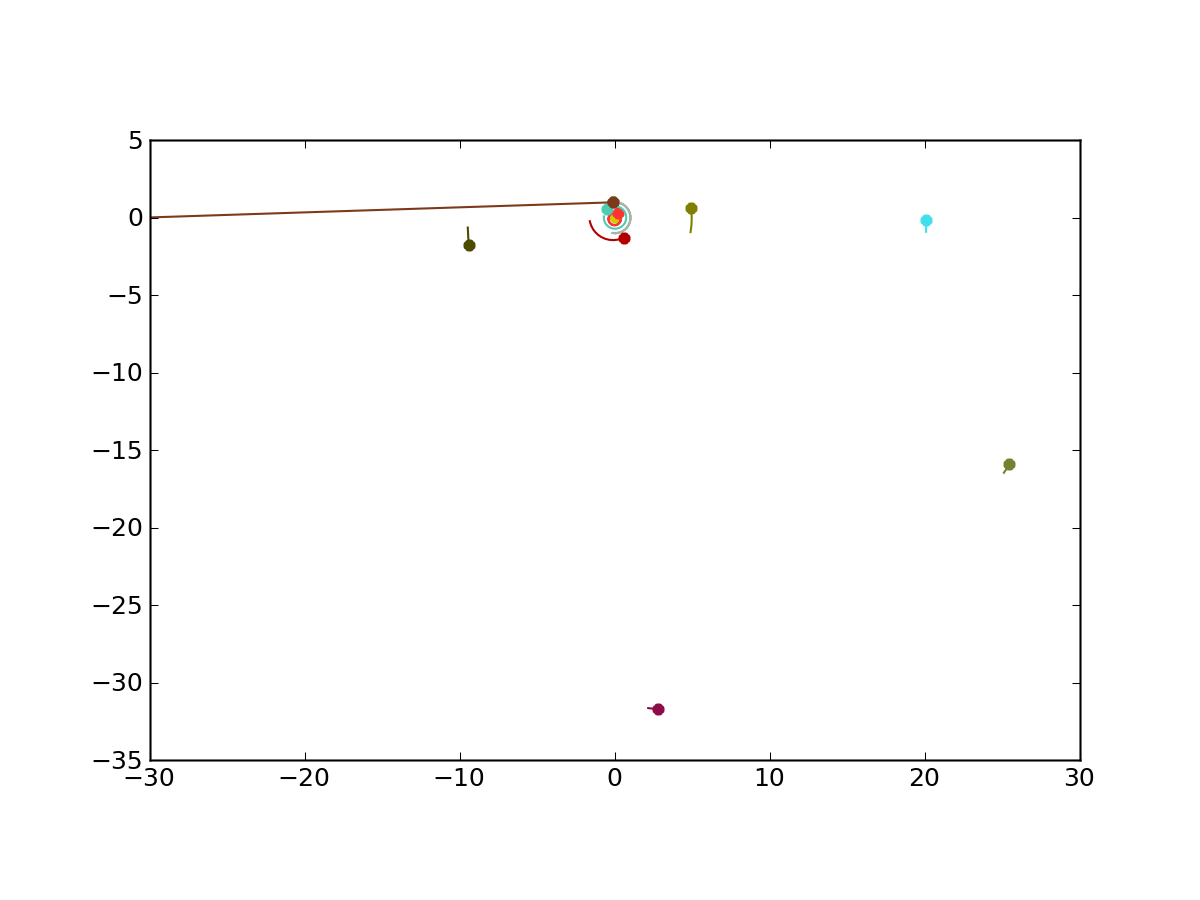
\includegraphics[scale=0.38]{img/torpedo/proyectilhit_all.png}
	\label{fig:res_misil_1}
	}
	\\
	\subfigure[Impacto zoom: 2.2]{
	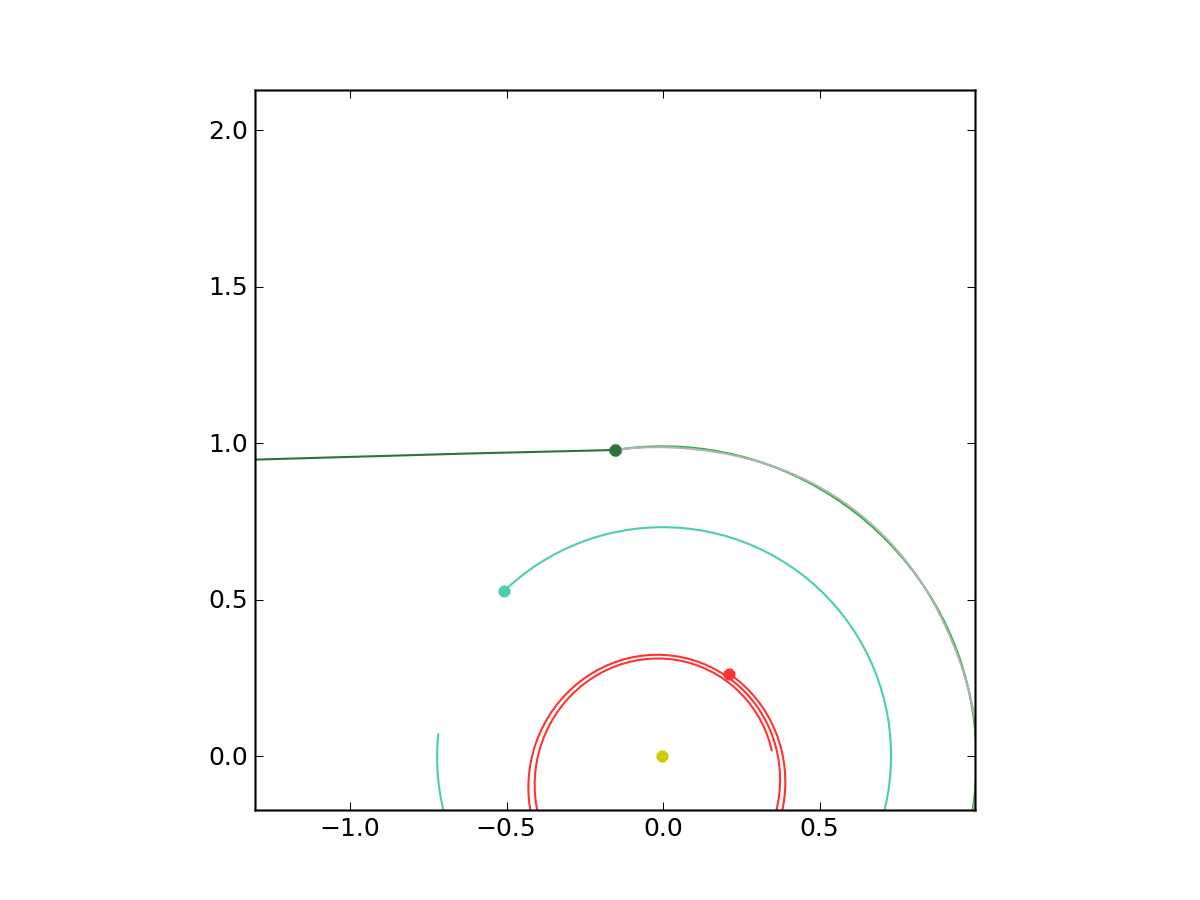
\includegraphics[scale=0.38]{img/torpedo/proyectilhit_zoom1.png}
	\label{fig:res_misil_2}
	}
	\subfigure[Impacto zoom: .2]{
	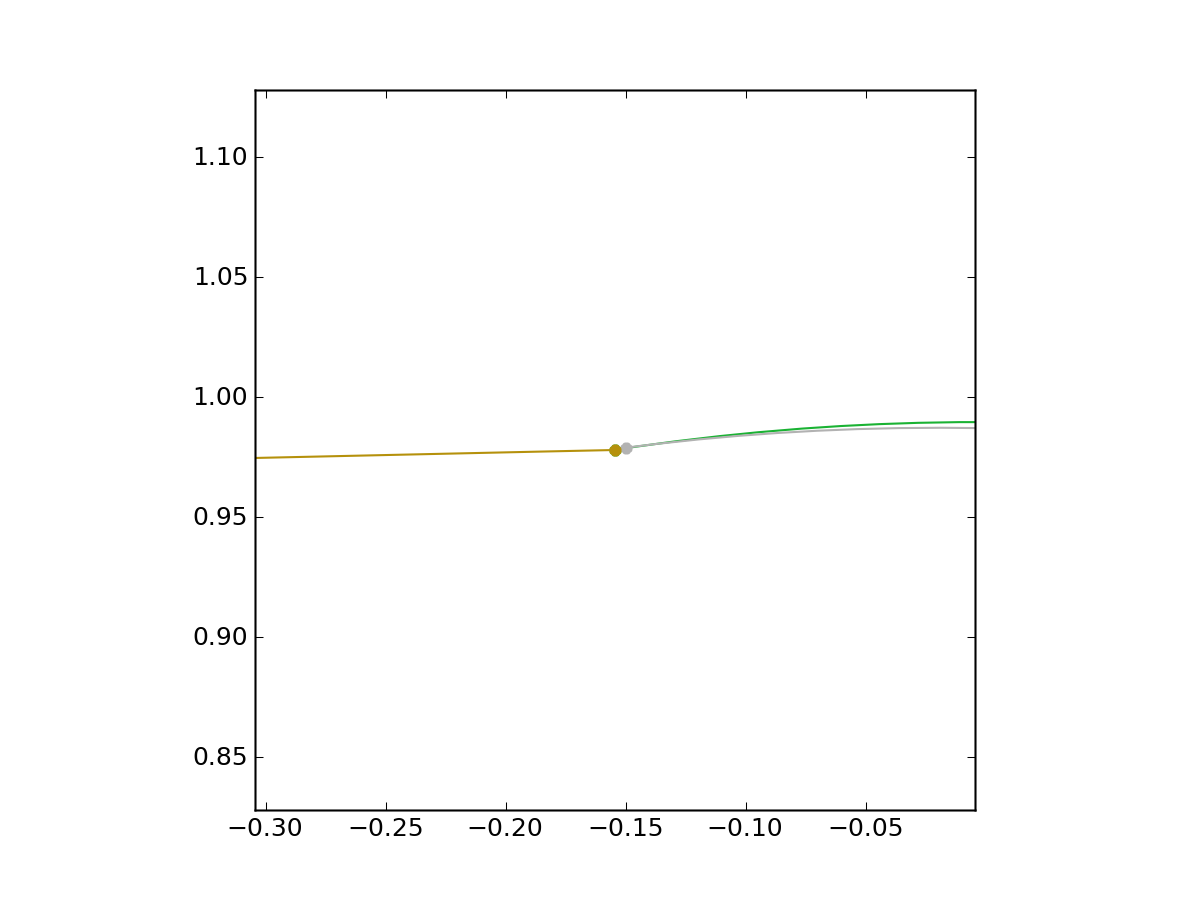
\includegraphics[scale=0.38]{img/torpedo/proyectilhit_zoom2.png}
	\label{fig:res_misil_3}
	}
	\caption{
		Acá vemos la simulación de el proyectil \textit{Torpedo de Protones} para una instancia en la que le pega a la tierra,
		con distintas ampliaciones.
		El misil fue disparado desde el punto $<-30,.005, 0>$ AU (aproximadamente) a una velocidad de $<0.147774,0.00480309,-3.62451e-08>$ AU/día.
	}
	\label{ fig:res_misil }
\end{figure}
